\documentclass{article}
\usepackage{graphicx} % Required for inserting images
\usepackage[utf8x]{inputenc}
\usepackage[english,russian]{babel}
\usepackage{cmap}
\usepackage{mathtools}
\usepackage{graphicx} %Вставка картинок правильная
\usepackage{float} %"Плавающие" картинки
\usepackage{wrapfig }%Обтекание фигур (таблиц, картинок и прочего)
\usepackage{geometry} % Отступы
\usepackage{pdfpages} % Для вставки других пдф страниц

\geometry{
  a4paper,
  top=30mm, 
  right=30mm, 
  bottom=30mm, 
  left=30mm
}

\newcommand{\RomanNumeralCaps}[1]
    {\MakeUppercase{\romannumeral #1}}

\title{Физика Зачет}

\begin{document}

\maketitle

\begin{enumerate}
    \item Магнитизм
    \begin{enumerate}
        \item Магнитные явления. Магнитное поле, свойства магнитного поля.  Закон Ампера для элемента тока и витка с током.
        \item Вектор магнитной индукции. Принцип суперпозиции полей. Закон Био-Савара-Лапласа. Индукция магнитного поля прямолинейного проводника с током, кругового витка и катушки с током.
        \item Взаимодействие прямолинейных проводников с током. Определение единицы силы тока в СИ.
        \item Сила Лоренца. Движение заряженных частиц в электрических и магнитных полях.
        \item Явление электромагнитной индукции. Закон Фарадея. Правило Ленца. ЭДС, возникающая в проводнике, движущемся в магнитном поле.
        \item Вихревые поля. Связь электрического и магнитного полей. Явление самоиндукции. Индуктивность, что характеризует, от каких параметров зависит.
        \item Индуктивность соленоида. Энергия магнитного поля соленоида. Плотность энергии магнитного поля.
        \item Магнитные свойства вещества. Диамагнетики, парамагнетики, ферромагнетики.
    \end{enumerate}
    \item Колебания
    \begin{enumerate}
        \item Колебательное движение. Условия возникновения колебаний. Параметры колебательного движения. Гармонические колебания.
        \item Колебания пружинного маятника. Превращения энергии в гармонических колебаниях.
        \item Математический маятник. Формула Гюйгенса. Превращения энергии в гармонических колебаниях.
        \item Физический маятник. Период свободных колебаний физического маятника.
        \item Сложение гармонических колебаний, происходящих по одной прямой и по двум взаимно-перпендикулярным направлениям. Фигуры Лиссажу.
        \item Вынужденные механические колебания. Резонанс. Резонансные кривые
    \end{enumerate}
    \item Переменный ток
    \begin{enumerate}
        \item Электромагнитные колебания. Колебательный контур. Формула Томсона.
        \item Переменный электрический ток. Рамка, вращающаяся в магнитном поле. Генератор переменного тока.
        \item Производство, передача и использование электроэнергии. Трансформаторы.
        \item Резистор в цепи переменного тока. Действующее значение ЭДС, напряжения и силы тока.
        \item Конденсатор в цепи переменного тока. Катушка индуктивности в цепи переменного тока.
        \item Вынужденные колебания в цепи переменного тока. Закон Ома для цепи переменного тока. Резонанс напряжений и токов.
        \item Мощность, выделяющаяся в цепи переменного тока.
    \end{enumerate}
    \item Волны
    \begin{enumerate}
        \item Механические волны. Виды волн и их характеристики.
        \item Уравнение бегущей волны. Плоские и сферические волны. 
        \item Принцип Гюйгенса. Законы отражения и преломления механических волн.
        \item Свойства волн. Интерференция волн. Условия минимума и максимума интерференции.  Дифракция волн. 
        \item Стоячая волна. Уравнение стоячей волны. Возникновение стоячей волны. Собственные частоты колебаний.
        \item Звуковые волны. Скорость звука.  Движение тел со скоростью большей скорости звука. Эффект Доплера в акустике.  
        \item Электромагнитные волны. Открытие электромагнитных волн - опыты Герца. Свойства электромагнитных волн. Перенос энергии электромагнитной волной. Шкала электромагнитных излучений. 
    \end{enumerate}
\end{enumerate}

\section{Магнетизм}
\begin{flushleft}
    \begin{itemize}
        \item Явления и свойства магнитного поля читать в Грачеве (стр 84, 17 - 18 параграф)
        \item Материя, по средствам которой осуществляется электромагнитные взаимодействия, называется магнитной индукцией.
        \item Закон Ампера: На элемент с током длины $\Delta l$ со стороны магнитного поля с индукцией $\Delta \overrightarrow{B}$, действует сила Ампера. \[\overrightarrow{F_a} = I [\overrightarrow{B} \times \overrightarrow{l}]\]
        \item Модуль силы Ампера $F_A = IlB \sin{\alpha}$
        \item Взаимодействие двух проводников с током $F_A = \frac{\mu_0 I_1 I_2 \Delta l} {2 \pi r}$
        \item Для характеристики магнитного поля вводится величина, которая называется вектор магнитной индукции $\overrightarrow{B}$. 
        \item Закон Био-Савара-Лапласа $\Delta \overrightarrow{B} = \frac{\mu_0}{4 \pi} I \frac{[\Delta \overrightarrow{l} \times \overrightarrow{r}]}{r^3}$; $\mu_0 = 4 \pi \cdot 10^{-7}$
        \item Для проводника с током $B = \frac{\mu \mu_0 I}{2 \pi r}$
        \item Для кругового витка $B = \frac{\mu \mu_0 I}{2R}$
        \item Для катушки $B = \mu \mu_0 nI; n = \frac{N}{l}$, N - кол-во витков в катушке, l - ее длина
        \item Вектор $\Delta \overrightarrow{B} \perp$ плоскости, к которой лежат вектора $\Delta \overrightarrow{l}$ и $\overrightarrow{r}$ и направлен таким образом, чтобы из его конца кротчайшее вращение $\Delta \overrightarrow{l}$ до вращение $\overrightarrow{r}$ происходило против часовой стрелки (По правилу Буравчика). 
        \item Принцип суперпозиции вектора магнитной индукции: \[ \overrightarrow{B} = \sum_{i = 1}^n \overrightarrow{B_i}\]
        \item Ампер = Кулон / Сек. Ампер - кол-во заряда проходящее за секунду через поперечное сечение проводника.
        \item Сила Лоренца: на движущиеся частицы магнитного поля действует сила Лоренца, которая определяется по формуле $\overrightarrow{F_\text{л}} = q[\overrightarrow{V} \times \overrightarrow{B}]$
        \[F_\text{л} = qVB \sin{\alpha}\]
        \item Если частицы движутся одновременно в эл. и магн. полях, то применяется обобщенная формула Силы Лоренца: \[\overrightarrow{F_\text{общ}} = \overrightarrow{F_\text{ку}} + \overrightarrow{F_\text{л}}\]
        \item Электромагнитная индукция - это явление, при котором магнитное поле в $\text{катушке}_\RomanNumeralCaps{1}$ индуцирует (создает) ток в $\text{катушке}_\RomanNumeralCaps{2}$.
        \item Закон Фарадея: ЭДС индукции в замкнутом контуре ровна и противоположна по знаку скорости изменения магнитного потока пронизывающий этот контур. $\epsilon_i = - \frac{\Delta \Phi_0}{\Delta t}$
        \item Правило Ленца: Возникающий в контуре индукционный ток имеет такое направление, чтобы своим магнитным полем препятствовать изменению магнитного потока, которым вызван индукционный ток.
        \item Если проводник перемещается в постоянном магнитном поле, то в нем появиться ЭДС индукции (по причине действия силы Лоренца, можно посмотреть лекцию Ришельевского лицея на тему силы Лоренца).
        \item Вихревое Электрическое Поле. Максвел открыл свойство природы - меняющиеся во времени магнитное поле меняет электрическое поле. Электрическое поле действует на заряд, создавая электрический ток. Линии возникшего электрического поля оказались замкнутыми вокруг линий магнитного поля (линий магнитной индукции). Поэтому этот ток назвали \textbf{вихревым}.
        \item Согласно идеям Максвелла, переменное магнитное поле всегда связано с порождаемым им электрическим полем. В свою очередь, переменное электрическое поле с порождаемым им магнитным полем. Таким образом, переменное электрическое поле и магнитное поле неразрывно связаны. Они образуют единое электромагнитное поле. (подробнее на "https://www.tooelu.ee/ru/113/elektromagnitnoe-pole")
        \item Оказывается, что электрический ток в контуре, меняющийся со временем, воздействует сам на себя. ЭДС магнитной индукции, возникающий в этом контуре, при изменении силы тока называется \textbf{ЭДС самоиндукции}.
        \item Физическую величину, равную отношению магнитного потока $\Phi$, порожденного током в контуре, через поверхность, ограниченную этим контуром, к силе тока $I$ в данном контуре, называют \textbf{индуктивностью контура} (или коэффициентом самоиндукции) \[L = \frac{\Phi}{I}\]
        Единица индуктивности в СИ - \textit{генри} (Гн); 1 Гн = 1 Вб / A
        \item Пусть длин соленоида равна $l$, площадь поперечного сечения витка равна $S$,число витков равно $N$, а сила тока в обмотке - $I$. Тогда, модуль индукции магнитного поля внутри соленоида $B = \mu \mu_0 nI; n = \frac{N}{l}$. Магнитный поток через поверхность, ограниченную одним витком, $\Phi_1 = B \cdot S$. Поскольку соленоид состоит из $N$ витков, общий поток $\Phi = N \cdot \Phi_1$. Следовательно, из формулы индуктивности получаем: \[L = \frac{\mu_0 \mu N^2 S}{l}\]
        \item Согласно закону Фарадея, новое ЭДС будет $\epsilon = - \frac{\Delta \Phi}{\Delta t} = -L \frac{\Delta I}{\Delta t}$
        \item Т.к. источник должен совершать работу по преодолению ЭДС самоиндукции, то тогда расчет такой работы позволяет получить формулу для вычисления энергии магнитного поля тока $I$, проходящего по цепи с индуктивностью $L$. \[W_\text{м} = \frac{LI^2}{2}\]
        \item Энергию магнитного поля можно вычислить, не только зная индуктивность цепи и силу тока в ней, но и зная модуль индукции магнитного поля. Расчеты показывают, что плотность энергии магнитного поля (энергия магнитного поля, приходящаяся на единицу объема) равна: \[\omega_\text{м} = \frac{B^2}{2 \mu \cdot \mu_0}\]
        \item По интенсивности взаимодействия с магнитным полем, все вещества делят на два класса: \textit{слабо магнитные} и \textit{сильно магнитные}. 
        \item Слабо магнитные - \textit{диамагнетики \emph{и} парамагнетики}.
        \item Сильно магнитные - \textit{ферромагнетики} и другие (подробнее - 24 параграф Грачев).
        \item Пусть $\overrightarrow{B_0}$ - индукция магнитного поля до заполнения его пространства магнетиком (в вакууме), а $\overrightarrow{B}$ наоборот, после заполнения. Тогда $\mu = \frac{B}{B_0}$ и называется это отношение \textit{магнитной проницаемостью вещества или среды}. Магнитные проницаемости диамагнетиков и парамагнетиков близки к 1 (У диамагнетиков $\mu$ < 1, у парамагнетиков $\mu$ > 1). У сильных магнетиков магнитная проницаемость существенно больше единицы и зависит от индукции внешнего поля (подробнее - 24 параграф Грачев). Примеры парамагнетиков: марганец, платина, алюминий... Диамагнетиками являются почти все газы (кроме кислорода и окиси азота), вода, серебро, золото, медь, алмаз, графит, свинец... Ферромагнетиками становятся многие сплавы железа, кобальта, никеля и ряда других веществ. Температура Кюри - температура при которой происходит переход магнетика из одного состояние в другое. 
    \end{itemize}
    \section{Колебания}
    \begin{itemize}
        \item Колебания - повторяющиеся во времени изменения состояние систем.
        \item Механические колебания - механическое движение тела или системы тел, которое повторяется во времени и происходит в окрестности положения равновесия.
        \item Положение равновесия - состояние системы, в котором она моет оставаться сколь угодно долго по времени.
        \item Амплитуда колебаний - величина его большего отклонения от положения равновесия.
        \item Период колебаний - время одного полного колебания.
        \item Частота колебаний - число периодических колебаний за единицу времени.
        \item Условия возникновения колебаний: 
            \begin{enumerate}
            \item Наличие у системы положения устойчивого равновесия.
            \item Отсутствие потери энергии за счёт действия силы трения.
        \end{enumerate}
        \item Гармоничные колебания - механические колебания, у которых координата изменяется по гармоничному закону.
        \\ Будем считать, что положение колебаний тела определяется координатой $\{x\}$, а положения равновесия - $x = 0$.
        \\ Тогда уравнение гармонических колебаний примет следующий вид: \[x'' + \omega^2 x = 0\] Решением такого уравнения является функция вида $x(t) = A\cos{\omega t + \varphi_0}$
        \item Пружинный маятник - механическая система, состоящая из пружины с коэффициентом упругости (жёсткости) $k$, один конец которой жёстко закреплён, а на втором находится груз массы $m$. $T = 2\pi \sqrt{\frac{m}{k}}$
        \item Математический маятник - небольшое тело подвешенное на невесомой нерастяжимой нити, размеры которой больше линейных размеров тела. $T = 2\pi \sqrt{\frac{l}{g}}$
        \item В процессе колебаний происходит переход энергии из кинетической в потенциальную (и наоборот), причем когда тело проходит положение равновесия $E_\text{К} = E_\text{макс}$, а в момент максимального отклонения $E_\text{П} = E_\text{макс}$. $E_\text{К}$ и $E_\text{П}$ находятся в противофазе.
        $E_\text{К} = \frac{mV^2}{2} = \frac{mA^2\omega^2}{2}sin^2(\omega t + \varphi_0) = 
        \frac{m(A\omega)^2}{4}(1 - \cos(2(\omega t + \varphi_0)))$
        \\$E_\text{П} = \frac{kx^2}{2} = \frac{kA^2}{2}cos^2(\omega t + \varphi_0); k = m\omega^2 =>$ \\
        $=> E_\text{П} = \frac{m(A\omega)^2}{4}(1 + \cos(2(\omega t + \varphi_0)))$
        $W_\text{мех} = E_\text{П} + E_\text{К} = \frac{m(V\omega)^2}{2}$
        \item Физический маятник - твёрдое тело, совершающее колебания под действием силы тяжести вокруг горизонтальной оси, не проходящей через центр инерции тела.
        \\ Док-во периода свободных колебаний напиши попозже, пока оставлю ссылку на док-во из инета https://studfile.net/preview/4548487/
        \item Сложения колебаний.
        \begin{figure}[H]
            \centering
            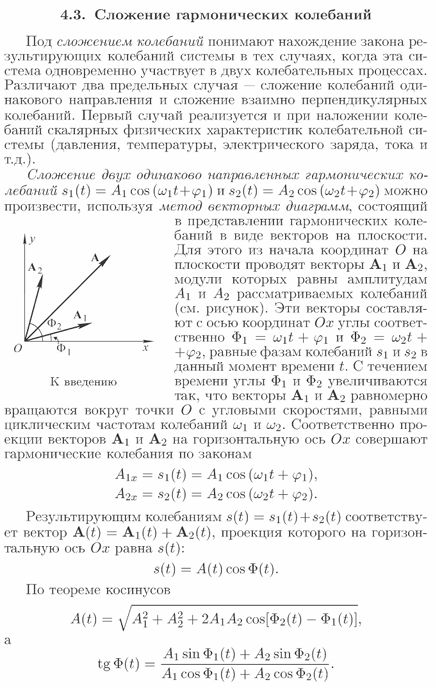
\includegraphics[width=0.5\linewidth]{images/Screenshot_1.png}
        \end{figure}
        \begin{figure}[H]
            \centering
            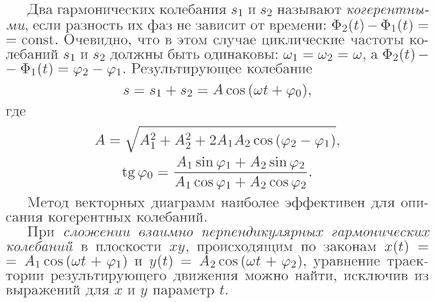
\includegraphics[width=0.5\linewidth]{images/Screenshot_2.png}
        \end{figure}
        % \begin{figure}
        %     \centering
        %     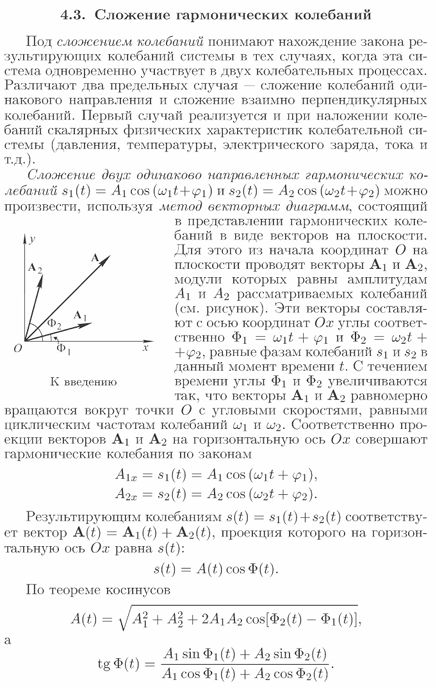
\includegraphics[width=0.5\linewidth]{images/Screenshot_1.png}
        %     \caption{Лягушка страницы 174 - 175}
        %     \label{fig:enter-label}
        % \end{figure}
        % \begin{figure}
        %     \centering
        %     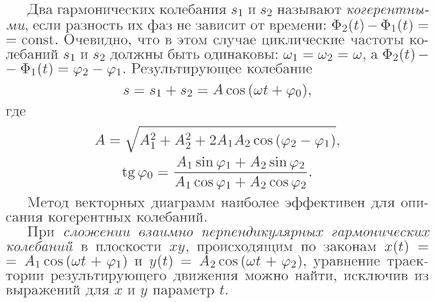
\includegraphics[width=0.5\linewidth]{images/Screenshot_2.png}
        %     \caption{Лягушка страницы 174 - 175}
        %     \label{fig:enter-label}
        % \end{figure}
        \item Фигуры Лиссажу - это замкнутые траектории, прочерчиваемые точкой, совершающей одновременно два гармонических колебания в двух взаимно перпендикулярных направлениях.
        \begin{figure}[H]
            \centering
            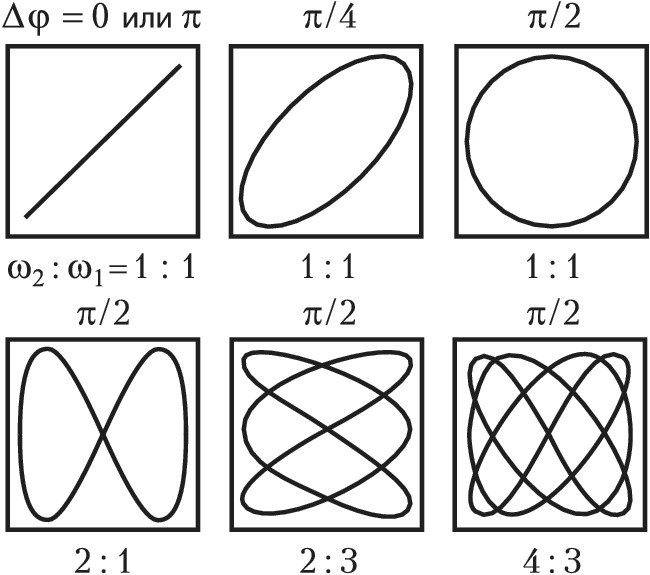
\includegraphics[width=0.3\linewidth]{images/FiguresLisaju.jpg}
            \label{fig:enter-label}
        \end{figure}
        \item Вынужденными механическими колебаниями называются колебания, совершаемые телом под действием внешней периодически изменяющейся силы. Вынуждающей силой является периодическая внешняя сила, влияющая на колебания. В примере с качелями вынуждающей силой является отталкивание качелей со стороны второго человека.
        \item Резонанс - это явление резкого возрастания амплитуды вынужденных колебаний при приближении частоты внешней силы, действующей на колебательную систему, к частоте собственных колебаний системы.
        \begin{figure}[H]
            \centering
            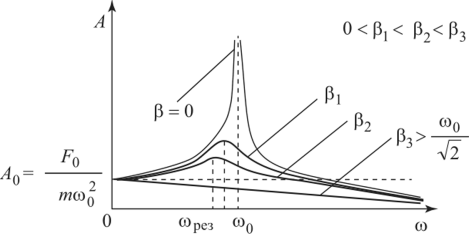
\includegraphics[width=0.4\linewidth]{images/Resonanse.png}
        \end{figure}
    \end{itemize}
    \section{Переменный ток и электромагнитные волны}
    \begin{itemize}
        \item Колебания, при которых энергия электрического поля преобразуется в энергию магнитного поля, называют электромагнитными колебаниями.
        \item Колебательный контур состоит из соединенных в замкнутую цепь конденсатора и катушки индуктивности. Зарядим конденсатор, после отключил ЭДС, подсоединив конденсатор к катушке. В результате образуется колебательный контур с начальным запасом энергии, равным  энергии заряженного конденсатора.
        \begin{figure}[h]
            \centering
            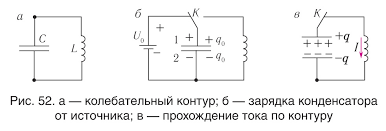
\includegraphics[width=0.5\linewidth]{images/Kontur.png}
            \label{fig:enter-label}
        \end{figure}
        Так как в начальный момент $t = 0$ на конденсаторе присутствовал начальный заряд $q_0$, а ток по цепе не шел, то начальная энергия системы была равна энергии на конденсаторе $W_0 = \frac{q_0^2}{2C}$. Пусть в некоторый момент времени $t_1$ заряд конденсатора и сила тока будут равны $q$ и $I$ соответственно. Тогда энергия магнитного поля, созданного током, будет равна $W_\text{магн} = \frac{LI^2}{2}$. Тогда полная энергия системы в какой то момент времени будет равна сумме этих двух энергий: \[W = W_\text{эл} + W_\text{магн} = \frac{q^2}{2C} + \frac{LI^2}{2}\]
        Если потери энергии колебательной системы пренебрежимо мыла, то ее энергия с течением времени остается неизменной, т.е. $W = W_0 = const$.
        Так же важно знать, что в любой момент времени сила тока в колебательном контуре равна производной по времени заряда пластины конденсатора. \[I = \lim\limits_{\Delta t\to 0} \frac{\Delta q}{\Delta t} = \dot q\]
        \item Уравнение гармоничных колебаний в замкнутом контуре: \[\ddot q + \frac{1}{LC}q = 0\]
        \item Формула Томсона: $\omega = \frac{1}{\sqrt{LC}}$; $T = \frac{2\pi}{\omega} = 2\pi \sqrt{LC}$ (Док-во читать в Грачеве параграф 38 стр 190)
        \item Электрический ток, сила которого с течением времени имезняется по гармоническому закону, называется переменным. \[\dot q(t) = I_m \cos(\omega t + \varphi_0)\]
        \item Рамка, вращающаяся в магнитном поле.
        \begin{figure}[H]
            \centering
            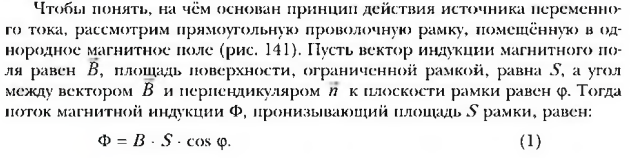
\includegraphics[width=0.8\linewidth]{images/Screenshot_3.png}
            \label{fig:enter-label}
        \end{figure}
        \begin{figure}[H]
            \centering
            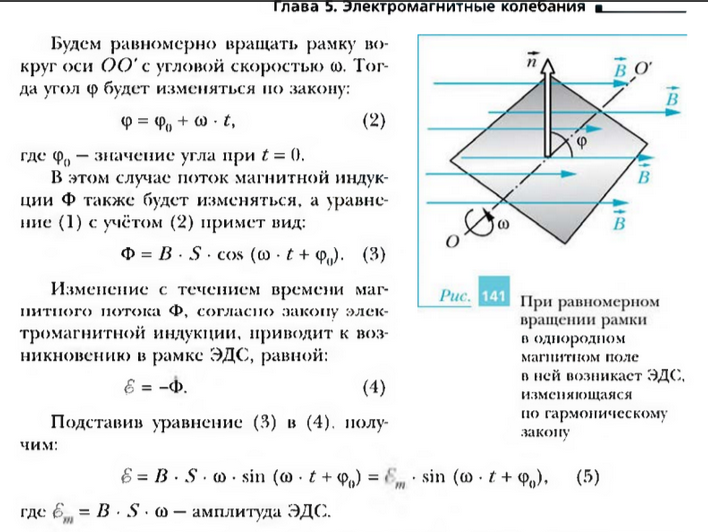
\includegraphics[width=0.8\linewidth]{images/Screenshot_4.png}
            \label{fig:enter-label}
        \end{figure}
        \item Генератор переменного тока - это источник тока, ЭДС которого меняется со временем. Таким, на пример, является, вращающаяся в магнитном поле (максимально подробно параграф 40 Грачев страница 198).
        \item Активное сопротивление в цепи переменного тока. \\ Рассмотрим цепь с конденсатором $R$ и источником тока, напряжение которого изменяется по гармоничному закону: \[U = U_m \cos(\omega t)\]
        В результате мы получаем вынужденные колебания в цепи. Определить I за короткий промежуток времени $\Delta t$ мы сможем с помощью формулы $I = \frac{U}{R}$ \[I = \frac{U_m}{R} \cos(\omega t) = I_m\cos(\omega t)\] $I_m = \frac{U_m}{R}$ - амплитуда силы тока. В данной цепи колебания напряжения и силы тока совпадают по фазе (синфазны).
        \item Мгновенная мощность $P = IU = I_m U_m \cos^2(\omega t)$, средняя мощность $\bar{P} = \frac{I_m U_m}{2}$
        \item Действующим или эффективным значением силы переменного тока называют силу такого постоянного тока, при котором мощность выделяющаяся в резисторе в цепи постоянного тока, равна средней за период мощности, выделяющейся в том же резисторе в цепи переменного тока. Аналагично с напряжением.
        \[\bar{P} = \frac{I_m U_m}{2} = I_\text{д} U_\text{д}\] \[I_\text{д} = \frac{I_m}{\sqrt{2}}\], \[U_\text{д} = \frac{U_m}{\sqrt{2}}\]
        \item Т.к.в резисторе $R$, включенном в данную цепь, выделяется мощность, отличная от 0, то его сопротивление $R$ часто называют активным сопротивлением. В общем случае, активным сопротивлением участка цепи переменного тока называют отношение средней за период мощности, выделяемой на этом участке, к квадрату действующего значения силы этого тока. \[R = \frac{\bar{P}}{I^2_\text{д}}\]
        \item Конденсатор в цепи переменного тока. \\Аналогично резистору подключим конденсатор в цепь переменного тока. В рассматриваемом случае напряжение на конденсаторе, равное разности потенциалов $U_c$ между его пластинами, в любой момент времени равно ЭДС источника: \[U_c = \mathcal{E}(t) = U_m \cos(\omega t) = \frac{q}{C}\]
        Тогда от сюда можно найти $q, I:$ \[ q = C U_m \cos(\omega t)\] \[I = \dot q = -I_m \sin(\omega t)\]
        \[U_m = I_m \frac{1}{\omega C}\]
        Колебания силы тока опережают по фазе колебания напряжения на конденсаторе на $\frac{\pi}{2}$.
        Вводится обозначение $X_c = \frac{1}{\omega C}$ - емкостное сопротивление этого конденсатора.
        \\Так же важным будет отметить, что различие фаз силы тока и напряжение приводит к тому, что мгновенная мощность переменного тока в течение периода изменяет знак. В результате среднее значение мощности, потребляемой конденсатором за период, равно нулю.
        \item Катушка индуктивности в цепи переменного тока. \\ Рассматриваем катушку индуктивности $L$ с пренебрежимо малым активным сопротивлением, сила тока в которой изменяется с течением времени по гармоническому закону: \[I = I_m \cos(\omega t)\] Возникающий ЭДС самоиндукции в катушке будет изменяться по закону: \[\mathcal{E} = -L \dot I = \omega LI_m \sin(\omega t)\] 
        В идеальной катушке напряженность вихревого электрического поля в каждой точке ее провода должна быть равна по модулю и противоположна по направлению напряженности электрического поля, обусловленного разностью потенциалов между выводами катушки. \[U = -\mathcal{E}\]
        Отсюда получаем напряжение между выводами катушки, изменяющееся с течением времени по закону: \[U = -\omega LI_m \sin(\omega t) = -U_m \sin(\omega t)\]
        Колебания напряжения на катушке опережают по фазе колебания силы тока в ней на $\frac{\pi}{2}$. Обозначим $X_L = \omega L$ - индуктивное сопротивление, тогда наша формула амплитудного значения напряжения примет вид $U_m = I_m X_L$.
        \\ Среднее значение мощности, потребляемой идеальной катушкой за период, равно нулю.
        \item Т.к. в реальности активное сопротивление отлично от нуля, RLC контур выделяет тепло, поэтому энергия магнитного поля теряется и колебания становятся затухающими. Для этого подключают источник питания. Частота установившихся вынужденных колебаний силы тока равна частоте изменения напряжения источника. Также, амплитуда установившихся вынужденных колебаний зависит от циклической частоты $\omega$ колебаний напряжения источника. Зависимость амплитуды установившихся колебаний от частоты называют амплитудно-частотной характеристикой (далее АЧХ). Частоту $\omega_\text{р} = \frac{1}{\sqrt{LC}}$, при которой амплитуда силы тока достигает максимального значения, называют резонансной частотой. Вид АЧХ колебательного контура зависит от активного сопротивления этого контура: чем меньше активное сопротивление, тем "острее" резонанс и, соответственно, больше максимальная амплитуда вынужденных колебаний, равная $I_{m \text{р}} = \frac{U_m}{R}$. 
        \begin{figure}[h]
            \centering
            \begin{subfigure}
                \centering
                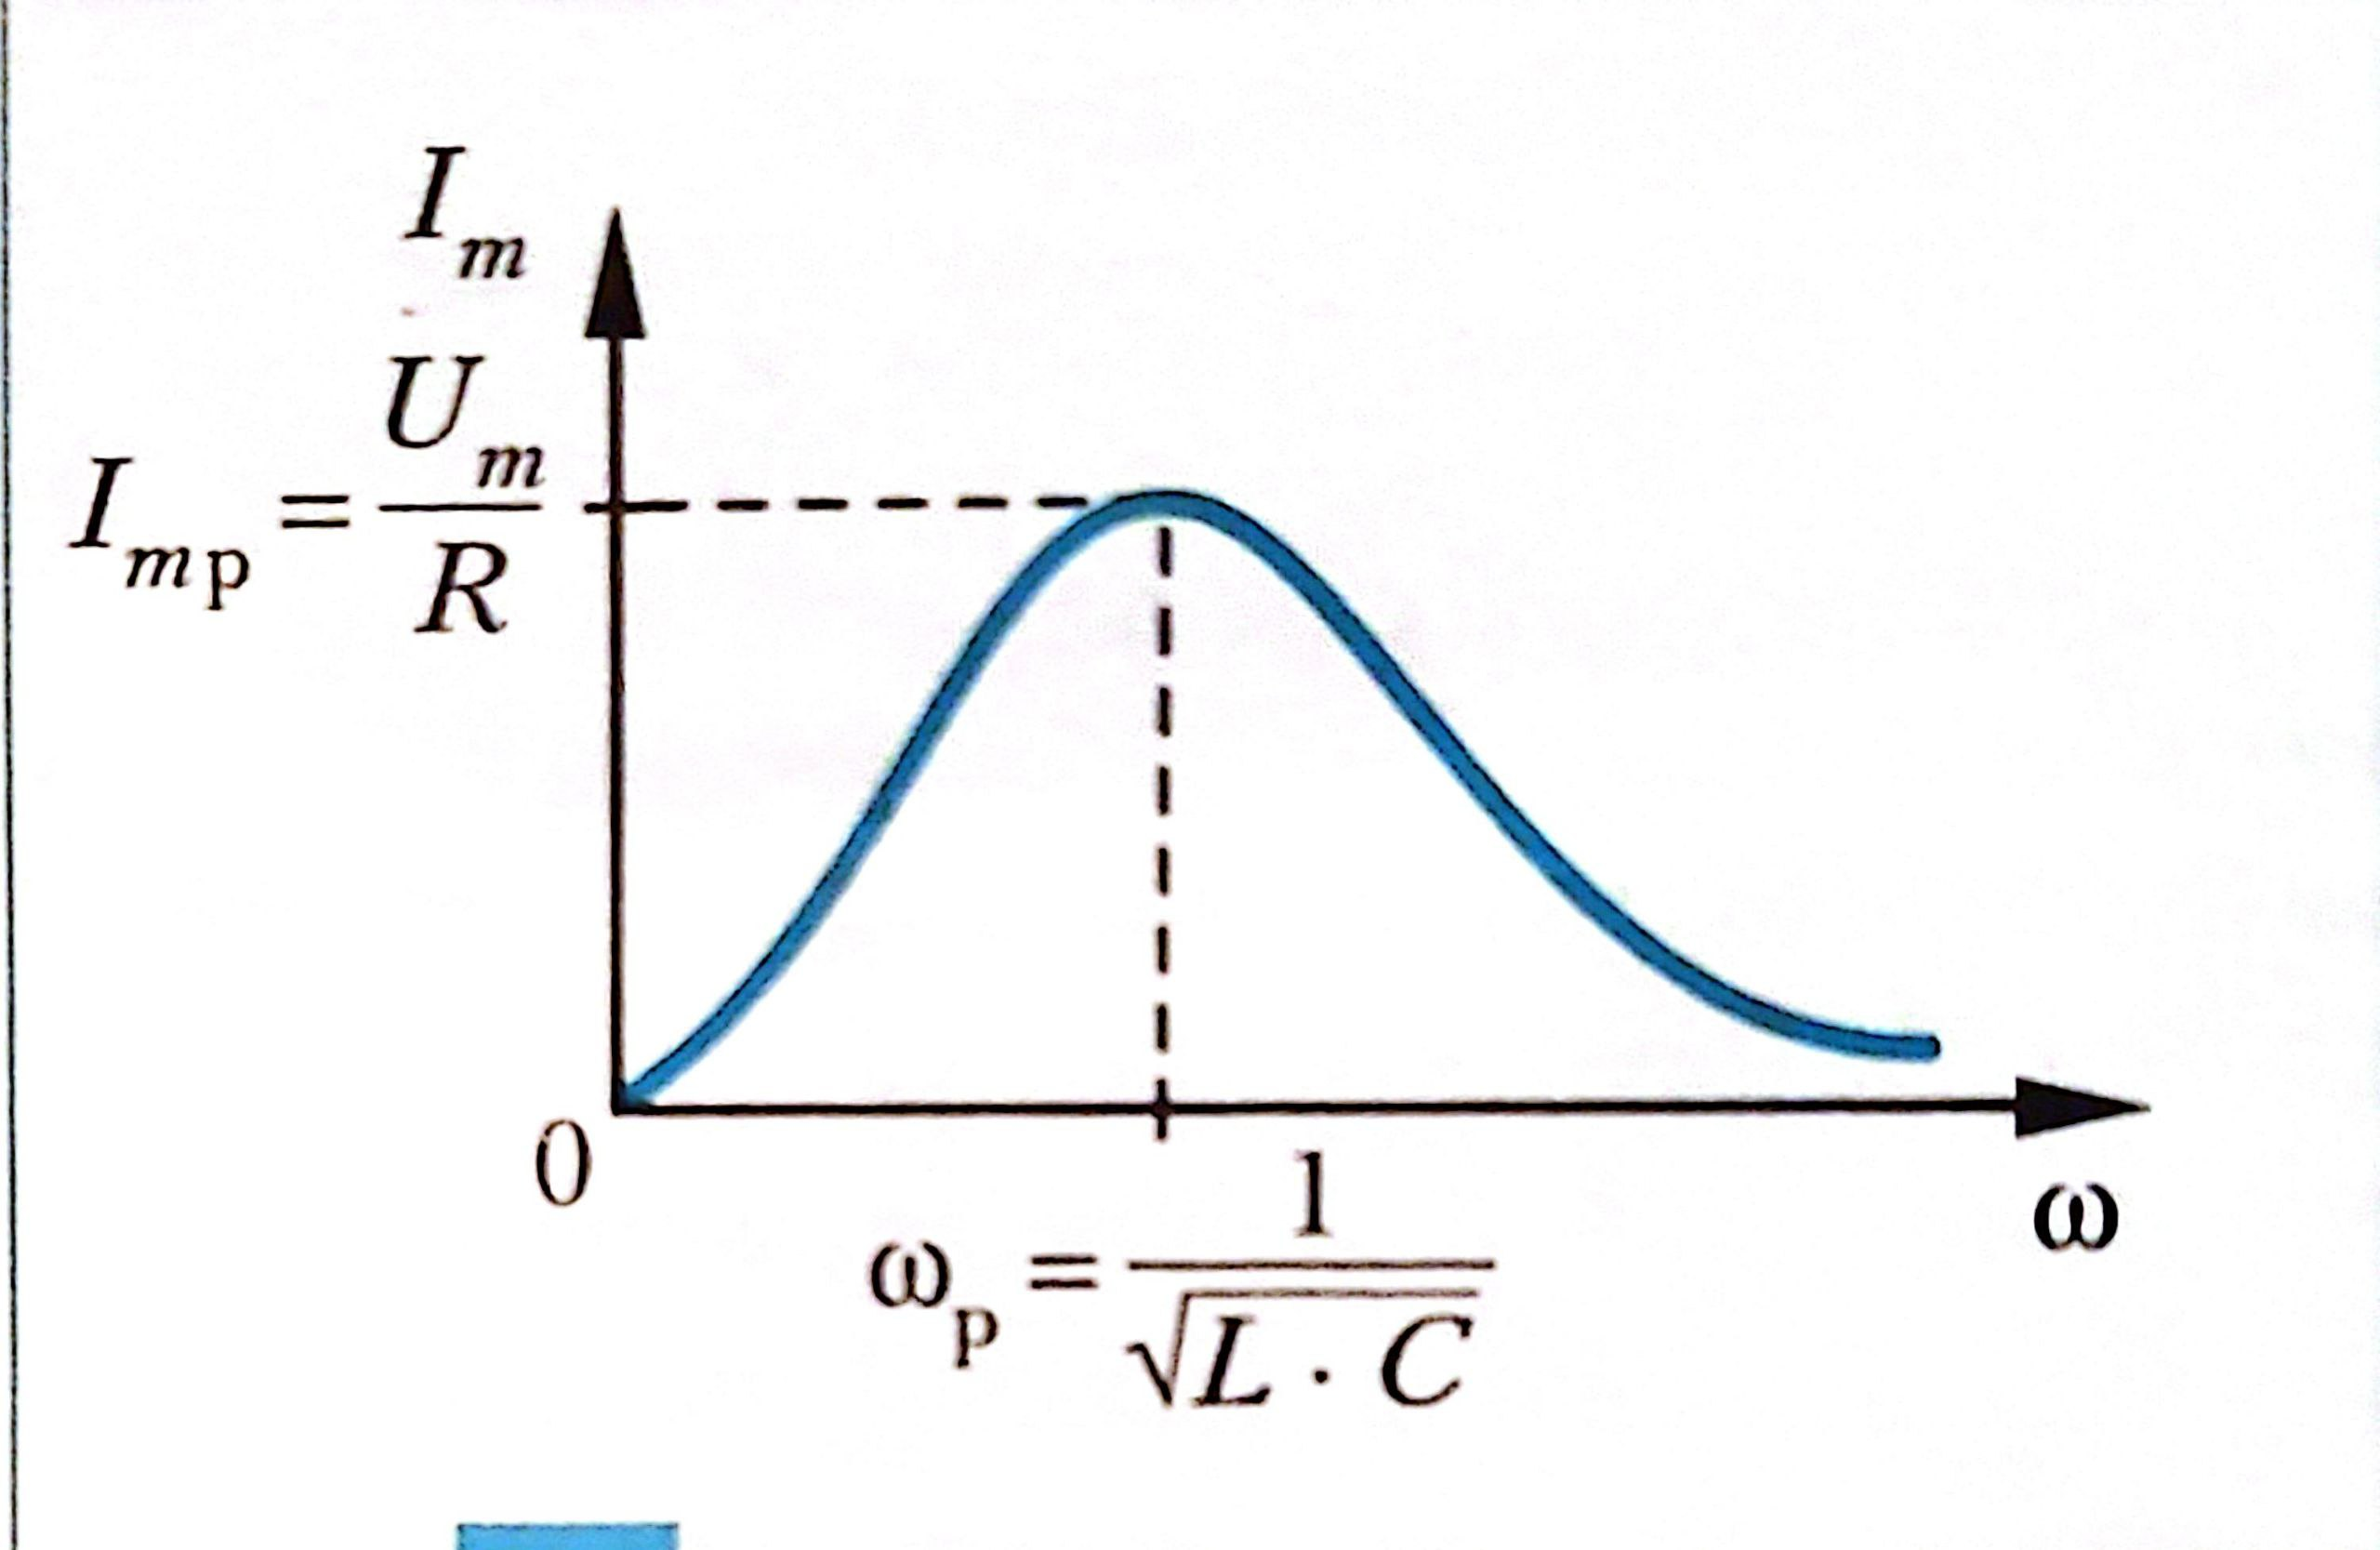
\includegraphics[width=.4\linewidth]{images/photo_2024-12-11_23-24-12.jpg}
                \label{fig:sub1}
            \end{subfigure}
            \begin{subfigure}
                \centering
                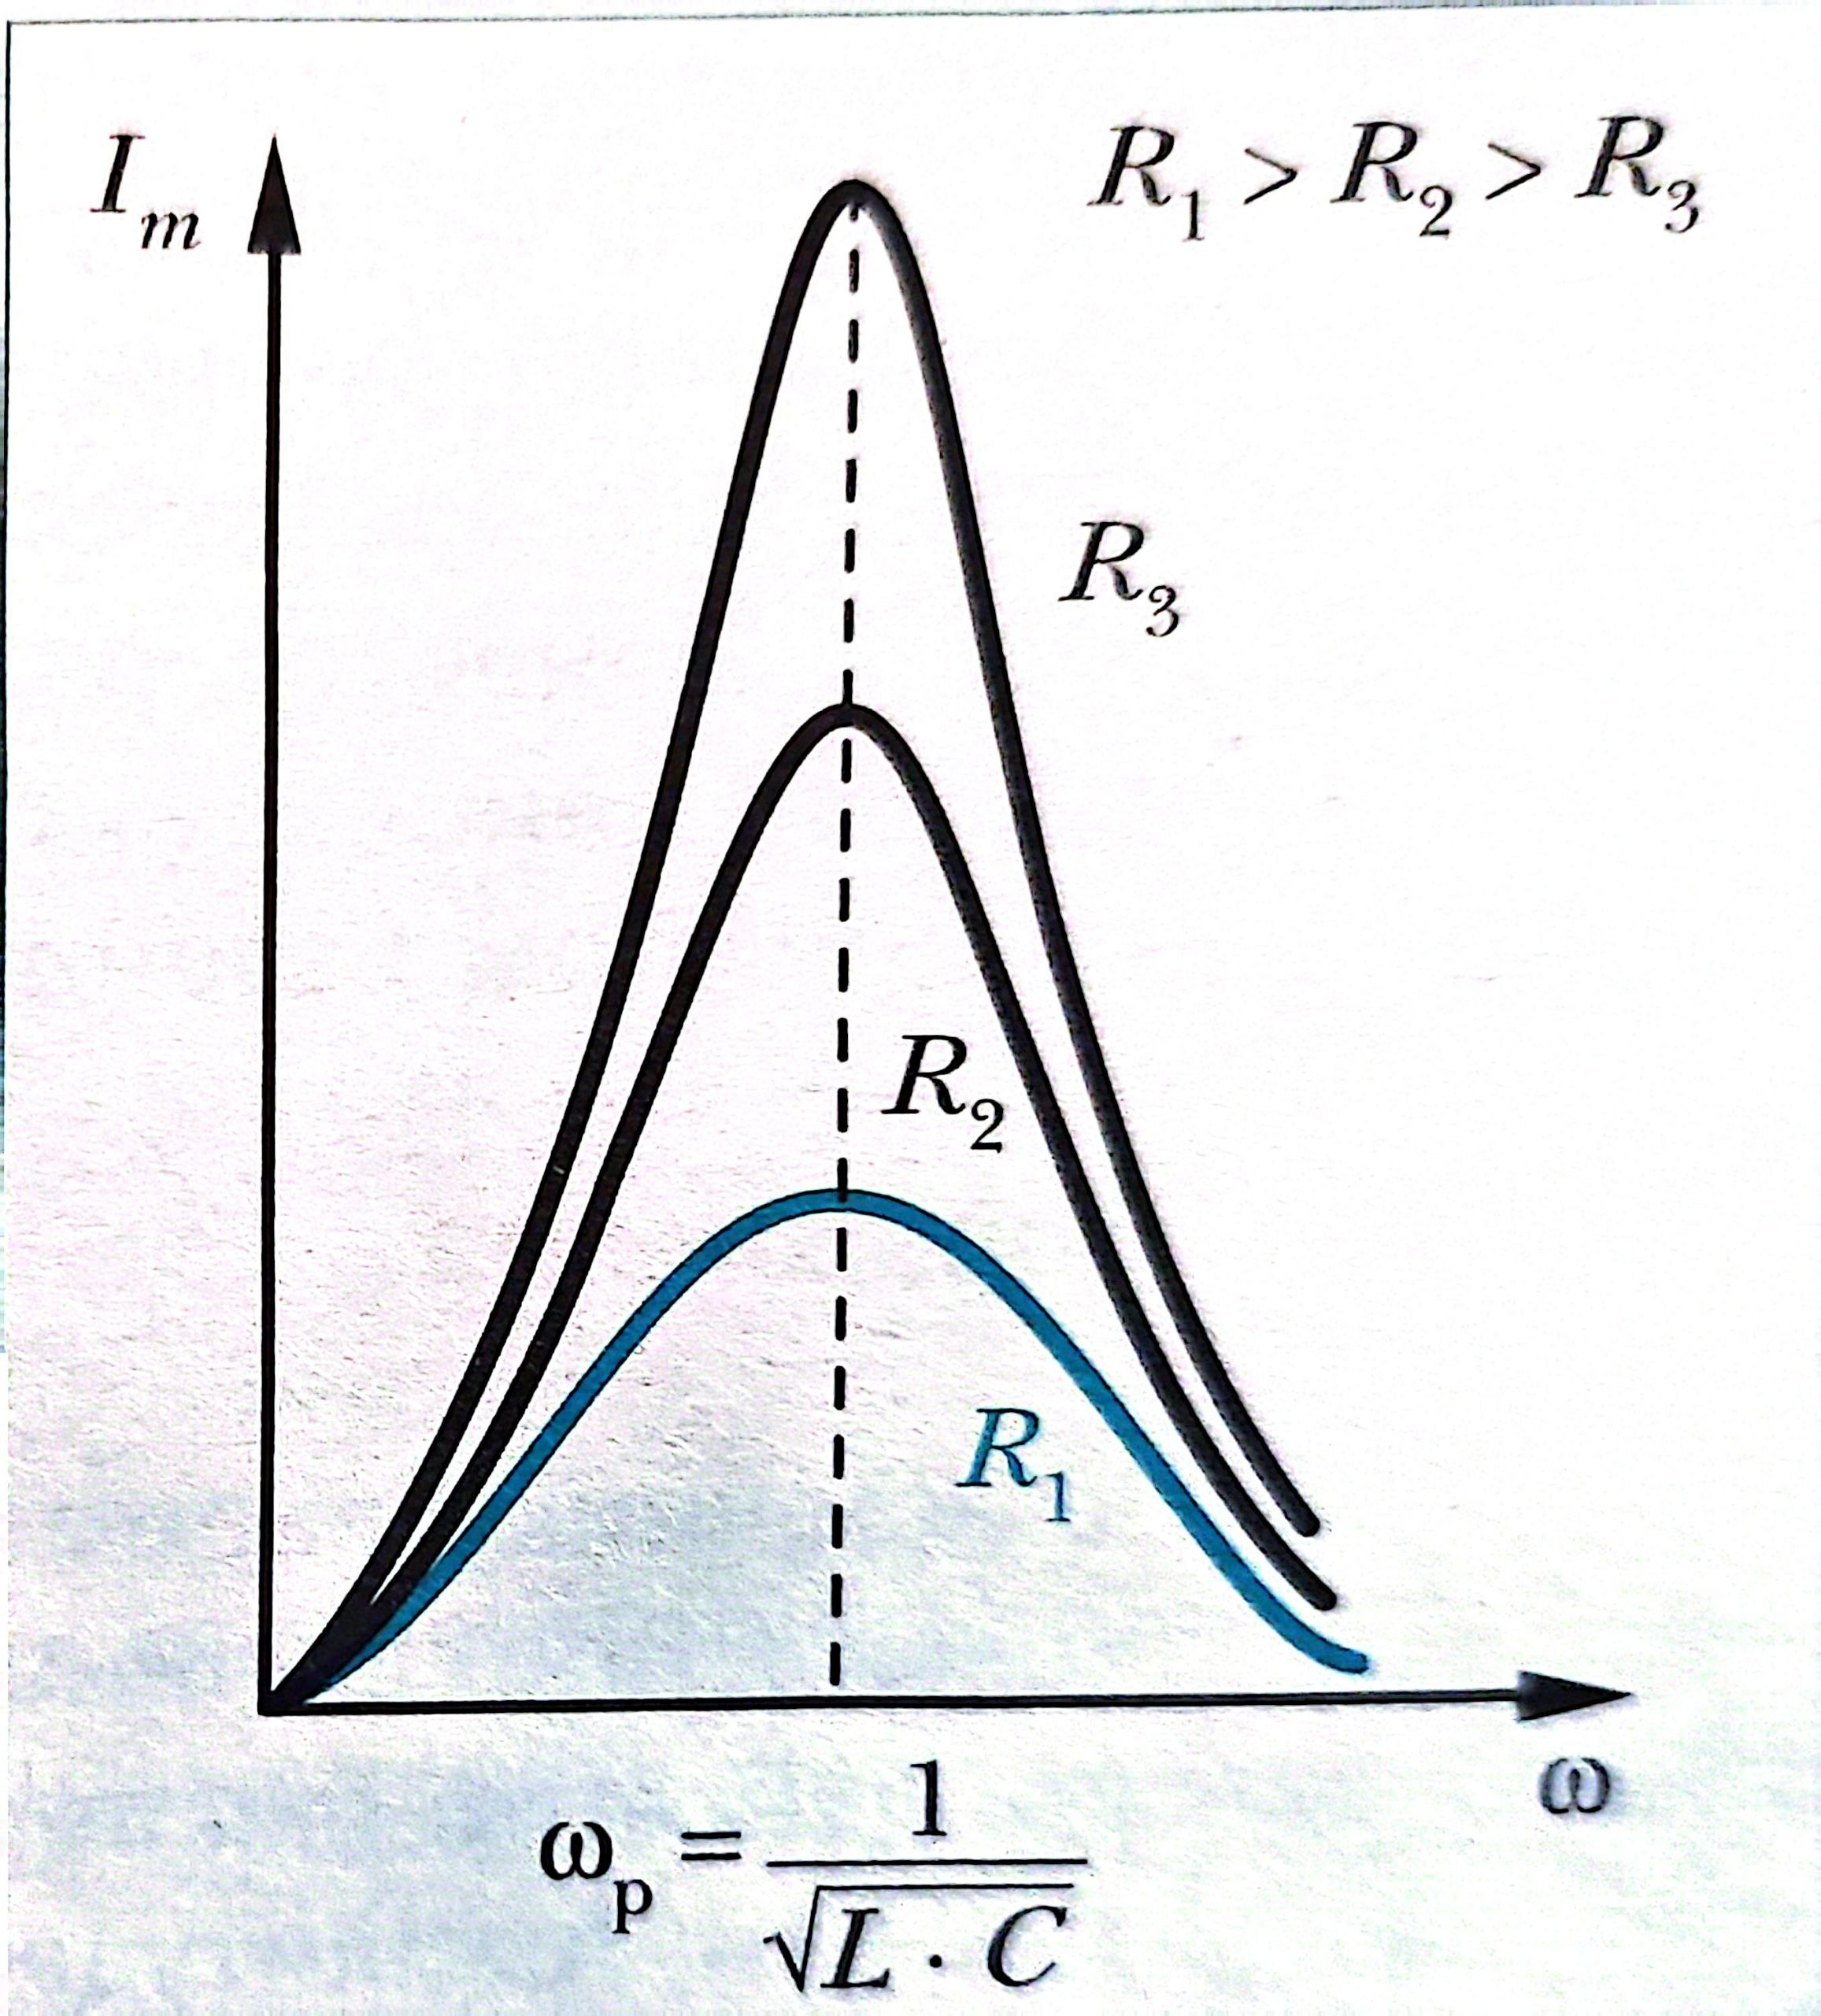
\includegraphics[width=.4\linewidth]{images/photo_2024-12-11_23-24-18.jpg}
                \label{fig:sub1}
            \end{subfigure}
        \end{figure}
        \item Закон ома для переменного тока.
        \\ Законы изменения напряжений на резисторе, конденсаторе и катушке индуктивности: \[
        U_R = I_m R \cos(\omega t)\]
        \[U_C = I_m X_C \cos(\omega t - \frac{\pi}{2})\]
        \[U_R = I_m X_L \cos(\omega t + \frac{\pi}{2})
        \]
        \[U = U_m \cos(\omega t + \varphi) = U_C + U_R + U_L\]
        Физическую величину $Z$, равную отношению амплитуды колебаний напряжения $U_m$ к амплитуде силы тока $I_m$, называют полным электрическим сопротивлением переменному току, а соотношение $U_m = I_m \cdot Z$ - законом Ома для цепи переменного тока. \[Z= \sqrt{(\omega L - \frac{1}{\omega C})^2 + R^2}\]
        \item Среднюю за период мощность $\bar{P}$ можно вычислить и через действующие значения силы тока и напряжения: \[\bar{P} = I_\text{д} U_\text{д} \cdot \cos(\varphi)\]
        $\cos{\varphi}$ -коэффициентом мощности.
        \\
        \textbf{ВАЖНАЯ ЗАМЕТКА}: в билетах переменного тока я не стал писать вопрос 17 и пару пунктов из вопроса о законе Ома. Их вы можете найти в учебнике Грачева. Достаточно прочитать 45 - 47 параграф, там глубоко и понятно затрагиваются эти темы. Желаю удачи на сессии. Про волны я не забыл, завтраа думаю напишу
    \end{itemize}
    \section{Волны}
    \begin{itemize}
        \item Распространяющиеся в упругой среде возмущения называют бегущими упругими волнами.
        \\В бегущей волне происходит перенос энергии в направление распространения волны и без переноса вещества.
        \\Возмущением называют выведенные части системы из положения равновесия.
        \\Волны, в которых колебания частиц происходят вдоль (перпендикулярно) направления (-ию) распространения самой волны, называют продольными (поперечными).
        \\Поверхностные волны - волны на поверхности жидкости.
        \item Скорость распространения этих возмущений называют скоростью волны.
        \\Расстояние, на которое распространяется волна за время, равное периоду колебаний, называют длиной волны $\lambda$. \[\lambda = v \cdot T\]
        \\Модуль скорости упругих продольных и поперечных волн зависит от упругих свойств среды и ее плотности. \[v = \sqrt{\frac{E}{\rho}}\]
        Где $E$ - модуль юнга материала тела, а $\rho$ - его плотность.
        \item Уравнение гармонической бегущей волны: \[y(x, t) = y_m \cdot \sin(\omega (t - \tau)) = y_m \cdot \sin(\omega (t - \frac{x}{v}))\]
        Используя выше приведенные формулы, это уравнение можно свернуть:
        \[y(x,t) = y_m sin(\omega t - kx)\]
        где $k = \frac{2\pi}{\lambda}$, называют волновым числом.
        \\Уравнение для сферических волн идентично, за исключением что амплитуда у них равна не $y_m$, а $\frac{y_m}{R}$. $R$ - расстояние от центра волны.
        \\ \textsc{ВАЖНО:} в жидкость и газах поперечные волны не распространяются.
        \item Плоские волны - волны, поверхности разных фаз которых представляют собой плоскости параллельные друг другу.
        \item Сферические волны - волны, поверхности равных фаз которых представляют концентрические сферы. Центры данных сфер называют центрами волн.
        \item Волновой фронт - геометрическое место точек в пространстве, до которых доходят возмущения к моменту времени $t$.
        \item Принцип Гюйгенса:
        \\ Каждая точка волнового фронта является вторичным источником сферических волн. Волновая поверхность результирующей волны в любой момент времени представляет собой результат интерференции огибающих вторичных волн. 
        \item Интерференция волн - явления их суперпозиции, при котором происходит во времени их взаимное усиление в одних точках пространства и ослабления в других. \\ При интерференции энергия колебаний передается в пространстве.
        \item Законы отражения и преломления механических волн:
        \begin{enumerate}
            \item Закон отражения волн: луч падающий, луч отраженный, перпендикуляр к границе раздела двух сред, восставленный в точке падения лежат в одной плоскости; угол падения равен углу отражения.
            \item Закон преломления волн: Луч падающий, луч преломлённый и перпендикуляр к границе раздела двух сред, восставленный в точке падения, лежат в одной плоскости; отношение синуса угла падения к синусу угла преломления есть величина постоянная для двух данных сред и называется относительным показателем преломления для двух данных сред.
        \end{enumerate}
        \item Показатель преломления: 
            \[
            \frac{sin{\alpha}}{sin{\gamma}} = \frac{n_2}{n_1} = \frac{v_1}{v_2} = n_{12}; v = \frac{c}{n}
            \]
        \item Условие минимума/максимума интерференции (для когерентных колебаний - имеющих одинаковую частоту): 
        \begin{enumerate}
            \item Амплитуда колебаний в некоторой точке интерференционной картины максимальна если разность фаз колебаний, создаваемых приходящими в эту точку волнами, равна:  \[
            \Delta \varphi = 2k \pi, k \in \mathcal{Z};
            \]
            В случае, когда источники волн синфазны, а модули скоростей распространения волн во всех направлениях одинаковы, условие интерференционных максимумов может быть записано в виде: \[
            \Delta l = k \lambda, k \in \mathcal{Z};
            \]
            Число $k$ называют порядком интерференции.
            \item Амплитуда колебаний в некоторой точке интерференционной картины минимальна, если разность фаз колебаний, создаваемых приходящими в эту точку волнами, равна: \[
            \Delta \varphi = (2k + 1)\pi,k\in \mathcal{Z};
            \]
            В случае, когда источники волн синфазны, а модули скоростей распространения волн во всех направлениях одинаковы, условие интерференционных минимумов может быть записано в виде: \[
            \Delta l = (2k + 1)\frac{\lambda}{2}
            \]
        \end{enumerate}
        \item Явления, обусловленные волновой природой света и приводящие к нарушению закона прямолинейного распространения света, называют дифракцией света. Дифракция свойственна волнам любой природы.
        \\Принцип Гюйгенса-Френеля: каждая точка, которой достигает первичная волна, становится источником вторичной волны, причем все такие вторичные источники являются когерентными. Колебания в произвольной точке - результат интерференции вторичных волн. (Эта формулировка из учебника, лучше ссылаться на нее)
        \item Стоячая волна — это волна, образующаяся при наложении двух бегущих волн, распространяющихся навстречу друг другу с одинаковыми частотами и амплитудами.
        \item Уравнение стоячей волны:
        \[
        y(x,t) = 2A\cos(\frac{2\pi}{\lambda}x)\cos{\omega t}
        \]
        \item Звуковыми волнами называют упругие волны с частотами от 16 Гц до 20 кГц. Упругие волны с частотами менее 16 Гц называют инфразвуковыми, а волны с частотами более 20 кГц - ультразвуковыми.
        \\ Для передачи звука необходимо наличие упругой среды между источником звука и его приемником.
        \\Для характеристики звука вводят специальные величины: громкость, высота тона и тембр.
        \\Громкость звука зависит от энергии приносимой звуковой волной и частоты звуковой волны. Чем больше частота чистого музыкального звука, тем выше его тон.
        \item Скорость звука - скорость распространения волны в среде. $c = 340 [\text{м/c}]$ (При $t$ = 20 градусов в воздухе)
        \item Движение тел со сверхзвуковой скоростью -
        \item Эффект Доплера в акустике:
        \\ Эффектом Доплера называется изменение частоты колебаний, воспринимаемой приемником, при движении источника этих колебаний и приемника друг относительно друга. Например, из опыта известно, что тон гудка поезда повышается по мере его приближения к платформе и понижается при удалении, т.е. движение источника колебаний (гудка) относительно приемника (уха) изменяет частоту принимаемых колебаний.
        \[
        \nu_\text{пр} = \nu_\text{ист}\frac{v + v_\text{пр}}{v - v_\text{пр}}
        \]
        (знаки + и - меняются местами при отдалении источника от приемника)
        \item Электромагнитные волны - поперечные колебания векторов напряженности электрического поля и магнитной индукции магнитного поля происходящие в плоскости перпендикулярной распространению заряда.
        Свойства: 
        \begin{enumerate}
            \item Электрические и магнитные поля - проявление единого электромагнитного поля.
            \item Изменяющиеся во времени токи и заряды, движущиеся с ускорением, могут является источником электромагнитных волн.
            \item Электромагнитное взаимодействие передается из точки А в точку Б не мгновенно, а с конечной скоростью. В вакууме скорость распространения электромагнитной волны равна скорости света: \[
            c = 3 \cdot 10^8 [\frac{\text{м}}{\text{с}}] = \frac{1}{\sqrt{\mathcal{E}_0 \mu_0}}
            \]
            или, если не в вакууме, то скорость света в среде равна: \[
            v = \frac{c}{\sqrt{\mathcal{E}\mu}}
            \]
            \item Электромагнитная волна является поперечной, то есть вектор напряжённости $E$ электрического поля и вектор магнитной индукции $B$ колеблются в направлении, перпендикулярном направлению распространения волны. При этом вектора $Е$ и $В$ колеблются синфазно в перпендикулярных направлениях.
            \begin{figure}[H]
                \centering
                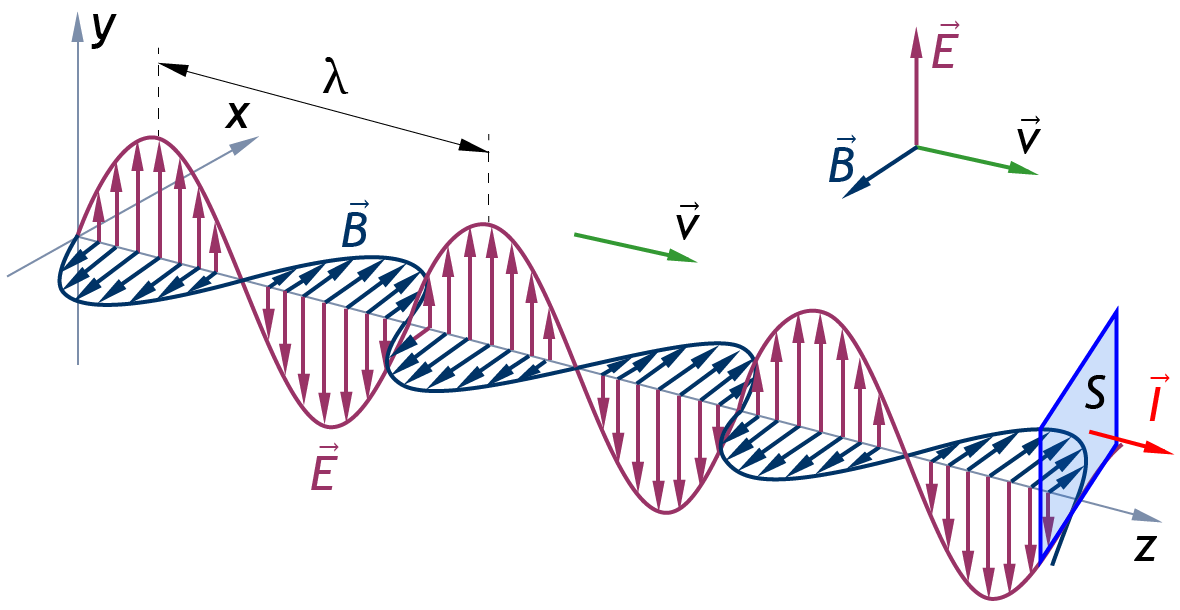
\includegraphics[width=0.5\linewidth]{images/348740.png}
                \label{fig:enter-label}
            \end{figure}
            \item Скорость электромагнитной волны в вакууме равна скорости света.\[
            c = 3 \cdot 10^8 [\frac{\text{м}}{\text{с}}]
            \]
            \item Эксперименты показали, что электромагнитные волны обладают теми же свойствами, что и механические волны: отражение, поглощение, преломление, интерференция и дифракция.
        \end{enumerate}
        \begin{figure}[H]
            \centering
            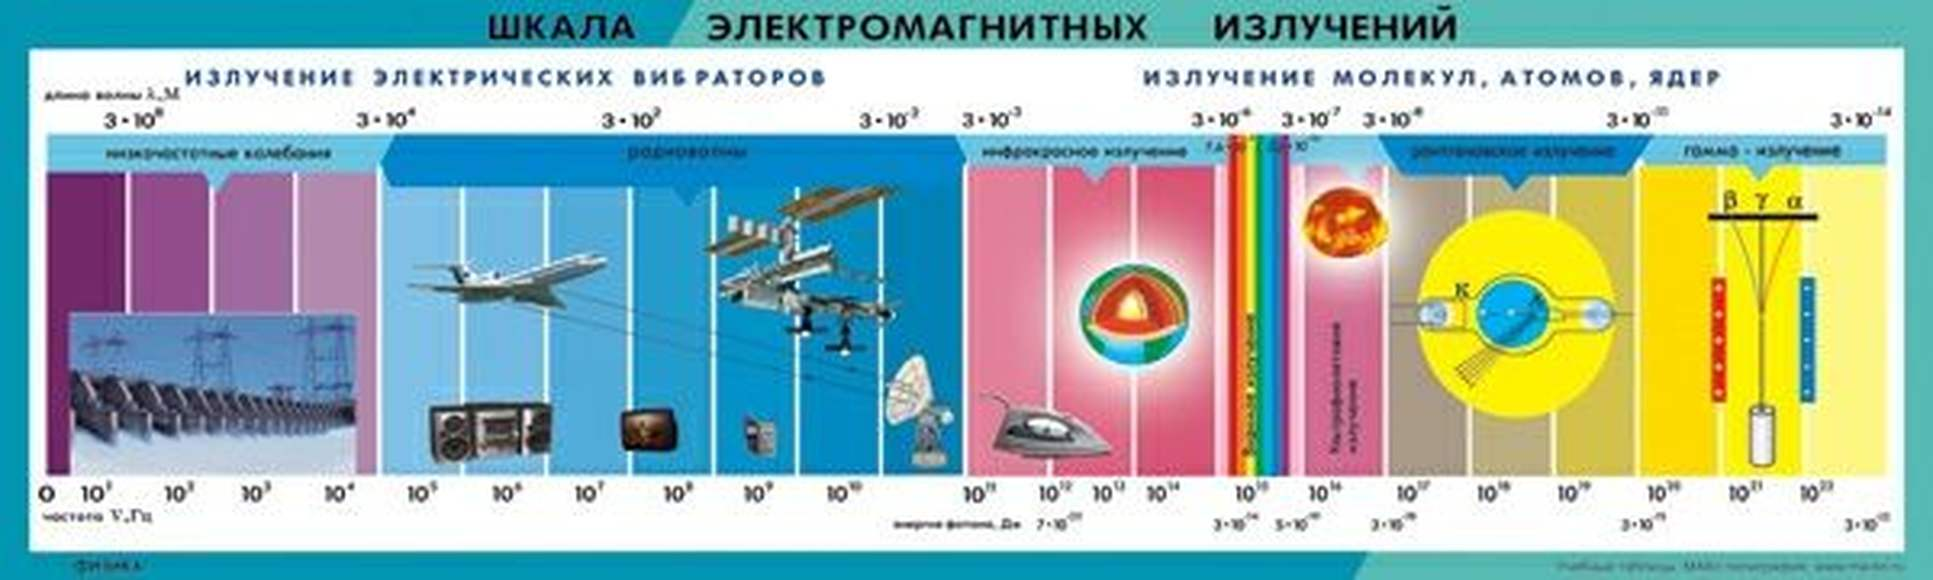
\includegraphics[width=0.9\linewidth]{images/637ad10a697b11ec9b2efa163e2f8b8d_f15b4d9a83ea11ec8c0ffa163e2f8b8d_auto_580_jpg_5_80.jpg}
            \label{fig:enter-label}
        \end{figure}
        \item Опыт Герца я всем, кому надо покидаю ссылку на видео, потому что как по мне так будет легче для всех, там ясно и понятно описывается суть опыта и все следствия.
    \end{itemize}
    \section{Заметка}
    \\Билеты пока не закончены, остались некоторые вопросы, которые я уточню на консультации. Если находите ошибки, большая просьба сообщать о них мне.
    \\Список недостающих, или не понятных на данных момент вопросов:
    \begin{itemize}
        \item Закон Ампера для витка с током.
        \item Энергия магнитного поля соленоида.
        \item Свойства волн (Поляризация).
        \item Собственные частоты колебаний.
        \item Скорость звука.
        \item Перенос энергии электромагнитной волной.
    \end{itemize}
\end{flushleft}
\end{document}
